%% 
%% ACS project dissertation template. 
%% 
%% Currently designed for printing two-sided, but if you prefer to 
%% print single-sided just remove ",two-side,open-right" from the 
%% \documentclass[] line below. 
%%
%%
%%   SMH, May 2010. 


\documentclass[a4paper,12pt,twoside,openright]{report}
\raggedbottom

%%
%% EDIT THE BELOW TO CUSTOMISE
%%

\def\authorname{Sean J.\ Parker\xspace}
\def\authorcollege{Clare Hall\xspace}
\def\authoremail{sjp240@cam.ac.uk}
\def\dissertationtitle{Model-based Reinforcement Learning in Computer Systems}
\def\wordcount{13533}

\usepackage{amsmath,amssymb}
\usepackage[ruled]{algorithm2e}
\usepackage{epsfig,graphicx,verbatim,parskip,tabularx,setspace,xspace,url,tikz,neuralnetwork,setspace,nicefrac,hyperref,booktabs}
\usepackage{caption,subcaption}
\usepackage{glossaries}
\usepackage[numbers]{natbib}

\def\UrlBreaks{\do\/\do-}

\makeglossaries

\newlength{\twosubht}
\newsavebox{\twosubbox}

\DeclareMathOperator*{\argmax}{arg\,max}
\DeclareMathOperator*{\argmin}{arg\,min}

\newglossaryentry{PPO}
{
    name=PPO,
    description={Proximal Policy Optimisation}
}

%% START OF DOCUMENT
\begin{document}


%% FRONT-MATTER (TITLE PAGE, DECLARATION, ABSTRACT, ETC) 
\pagestyle{empty}
\singlespacing
\input{titlepage}
\onehalfspacing
\input{declaration}
\newpage
{\Huge \bf Acknowledgements}\\

I would like to thank my supervisor, Dr. Eiko Yoneki, for constructive suggestions during the preliminary stages of this research. Furthermore, I would like to thank Sami Alabed for his continual feedback, advice and support throughout this project. Finally, I would also like to thank Sara for her invaluable support throughout the project, as well as her proof-reading and comments of this report.

\newpage

\textbf{Word Count: 13533}

\newpage
{\Huge \bf Abstract}
\vspace{24pt} 

This project investigates the use of model-based reinforcement learning (RL) in the domain of computer systems, specifically, that of optimising deep learning models by transforming the deep learning model which is represented as a computation graph. We aim to minimise the runtime cost on hardware devices by using an RL agent to choose a sequence of transformations and locations which mutate the graph. Recent work has aimed to apply reinforcement learning to computer systems with some success, especially with using model-free RL techniques. However, more recently, model-based methods has seen an increased focus of research as model-based reinforcement learning can be used to learn a model of the environment, that can be leveraged to train an agent inside the learned world-model---increasing sample efficiency. Furthermore, when using a hallucinogenic world model as the environment, rollouts can occur safely in parallel and, especially in systems environments, it circumvents the possible latency impact of stepping a system environment that can take orders of magnitude longer to perform an action compared to a video game emulator. This dissertation examines both the prior work for optimising deep learning models and the applicability of reinforcement learning to the problem.

\vspace*{\fill}


\pagenumbering{roman}
\setcounter{page}{0}
\pagestyle{plain}
\tableofcontents
\printglossary[title=List of abbreviations]
\listoffigures
\listoftables

\onehalfspacing

%% START OF MAIN TEXT 

\chapter{Introduction}

Services we often take for granted, such as web search, social networks and language translators, are composed of complex systems. Modern services have components that are underpinned by machine learning (ML) models, specifically, deep neural networks (DNN). Over the past decade there has been a focus on developing frameworks that provide tools using which we can design, train and evaluate these deep learning models.

A common internal representation for neural networks inside deep learning frameworks is that of a computation graph---a directed acyclic graph where nodes represent a specific computation and edges the paths where data is transferred. Frameworks such as TensorFlow \cite{tensorflow2015-whitepaper} and PyTorch \cite{pytorch} automatically apply optimisations in an effort to reduce computation resources during inference.

Currently, the optimisation in deep learning frameworks is performed using manually defined heuristics. For example, TensorFlow \cite{tensorflow2015-whitepaper} uses 155 handwritten optimisations composed of 53,000 lines of C++. While such heuristics are applicable for current architectures, network design is consistently evolving. Therefore, we require consistent innovation to discover and design rules that control the application of optimisations with guarantees that strictly improve efficiency. Eliminating the need for manual engineering work that is required to design and implement the heuristics for applying optimisations is a primary focus of this work.

Recent work, namely TASO by \citet{jia2019taso,jia2019optimizing} has shown it is possible replace the heuristics with a cost-based search. However, such approaches may not fully explore the potential search space due to the lack of forward planning in cost-based optimisation. As a step towards resolving the issue of poor exploration, this work explores the use of reinforcement learning (RL). RL is an area of machine learning in which an agent learns to act optimally, given a state and a suitable reward function, through interactions with an environment.

%This work focuses on the use of RL for the task of optimising computation graphs, the internal representation of neural networks in ML frameworks, in order to reduce on-device runtime.

In this work, we focus on the use of RL for the task of optimising deep learning graphs. Specifically, we focus on a model-based reinforcement learning which aims to learn a model of the environment in which they act. In our work, the network learns to model the dynamics of sub-graph transformations in a deep learning model as well as the impact on overall runtime of the model when executed on-device. Further, learning a model of the environment provides important benefits; for example, lookahead planning, low-cost state prediction and faster wall-clock training. We examine the use of world-models for learning the environment as well as training a controller inside a world model which removes the need of an expensive, time-consuming computer system to apply our chosen graph transformations.

This dissertations key contributions are:

\begin{itemize}
  \item Applies modern reinforcement learning approaches that eliminates the need for human engineered graph optimisations in machine learning frameworks. We show that our proposed method can improve runtime by up to 58\% compared to current deep learning frameworks and up to 10\% compared to the state-of-the-art.
  \item Provides a detailed discussion and analysis of our solution as well as comparison to the current state-of-the-art methods in published literature.
  \item Implemented a model-based RL agent (section \ref{sec:rlopt:subsec:mb-agent}), and environment (section \ref{sec:prob:subsec:sysenv}), for jointly choosing the optimal substitution and substitution location (section \ref{sec:prob:subsec:sap}).
  \item This work, to the best of our knowledge, is the first that has applied model-based reinforcement learning in optimising computation graphs to reduce hardware resource requirements.
\end{itemize}

The rest of the dissertation is structured as follows. Chapter 2 provides a background for computation graphs and the representation of deep learning models, reinforcement learning---both model-free and model-based---in the context of computer systems. Chapter 3 concretely introduces the optimisation problem and formulates the problem in the context of reinforcement learning. Furthermore, we also describe our approach for applying reinforcement learning to optimise the computation graphs as well as learning an accurate model of the environment. Chapter 4 covers the evaluation setup, our experiments and results for different methodologies. Finally, in chapter 5 we conclude the dissertation with a summary of our findings and discuss potential future work.
\pagenumbering{arabic} 
\setcounter{page}{1} 

\chapter{Background and Related Work}
% In this chapter, we detail the background and prior research that underpins the work described in later chapters. Further, we include an explanation of the theoretical concepts, both reinforcement learning and graph neural networks, which we have used extensively in this work.

\section{Introduction to Deep Learning Models}
This section discusses the way in which machine learning models are represented for efficient execution on physical hardware devices. First, we discuss how the mapping of tensor operations to computation graphs is performed followed by an overview of recent approaches that optimise computation graphs to minimise execution time.

Over the past decade, there has been a rapid development of various deep learning architectures that aim to solve a specific task. Common examples include convolutional networks (popularised by AlexNet then ResNets, etc), transformer networks that have seen use in the modelling and generation of language. Recurrent networks that have shown to excel at learning long and short trends in data.

Importantly, the fundamental building blocks of the networks have largely remained unchanged.  As the networks become more complex, it becomes untenable to manually optimise the networks to reduce the execution time on hardware. Therefore, there is extensive work in ways to both automatically optimise the models, or, alternatively apply a set of hand-crafted optimisations.

Computation graphs are a way to graphically represent both the individual tensor operations in a model, and the connections (or data-flow) along the edges between nodes in the graph. Figure \ref{fig:bg:perceptron} shows how the expression, $y = \texttt{ReLU}(\mathbf{w} \cdot \mathbf{x} + b)$, can be represented graphically in a computation graph.

\begin{figure}[ht]
  \centering
  \includegraphics[width=0.75\columnwidth]{sections/2background/images/bitmap}
  \caption[Single perceptron as a dataflow (computation) graph]{The operations shown in purple are the nodes of the computation graph which take an arbitraty number of inputs, performs a computation at the node and produces an output. The blue nodes represent the input nodes for tensors. The directed edges show the flow of tensors through the graph.}
  \label{fig:bg:perceptron}
\end{figure}

Similarly, the whole model can be converted into a stateful dataflow graph in this manner. By using a stateful dataflow (or computation) graph, we can use any optimisation technique for backpropagation of the model loss though the graph [TODO rewrite last sentence]. We consider two key benefits of this representation. First, we can execute the model on any hardware device as the models have a single, uniform representation. Secondly, it allows for pre-execution optimisations based on the host device, for example, we may perform different optimisations for executing on a GPU compared to a TPU.

\subsection{Current approaches to optimising deep learning models}

Due to the prevalence and importance of machine learning, especially deep networks, there is a focus on finding ways decrease the inference runtime and by extension, increasing the model throughput. All major frameworks such as Tensorflow \cite{tensorflow2015-whitepaper}, PyTorch \cite{}, MXNet, and Caffe have some level of support for performing pre-execution optimisations. However, the process of performing such optimisations is often time-consuming and cannot be completed in real-time. Rather, it is to use a deep learning optimisation library such as cuDNN \cite{chetlur2014cudnn}.

%common machine learning framework is designed to greedily apply a set of pre-defined substitutions to an input graph in an attempt to optimise the graph. Tensorflow made use of low-level libraries such as cuBLAS \cite{cublas2008} for optimised matrix operations and cuDNN \cite{chetlur2014cudnn} for convolutional kernels. Furthermore, Tensorflow also contains a set of 155 substitutions that are implemented in 53,000 lines of code; to complicate matters, new operators are continuously proposed, such as grouped or transposed convolutions, all of which leads to a large amount of engineering effort required to maintain the library.

%TensorRT \cite{tensorrt2017} provides a high-performance SDK to optimise the inference of models via a combination of techniques such as layout and tensor fusion, auto-tuning kernels, and multi-stream execution. The SDK acts as both the optimisation and execution engine that lies between the ML framework and physical hardware. Importantly, it is not involved during the training process, rather, it assumes for the best possible performance that the developer 
TVM

Metaflow and TASO

\section{Reinforcement Learning}
Reinforcement learning (RL) is a sub-field in machine learning, broadly, it aims to compute a control policy such that an agent can maximise its cumulative reward from the environment. It has powerful applications in environments where a model that describes the semantics of the system are not available and the agent must itself discover the optimal strategy via a reward signal. Formally, RL is a class of learning problem that can be framed as a Markov decision processes (MDP) when the MDP that describes the system is not known \cite{bellman1957}; they are represented as a tuple $\langle \mathcal{S}, \mathcal{A}, \mathcal{P}_a, \mathcal{R}_a \rangle$ where:

\begin{itemize}
  \item $\mathcal{S}$, is a finite set of states
  \item $\mathcal{A}$, is a finite set of actions
  \item $\mathcal{P}_a$, is the state transition probability that an action $a$ in state $s_t$ leads to a state $s'_{t+1}$
  \item $\mathcal{R}_a$, is the reward from the environment after taking an action $a$ between state $s_t$ and $s'_{t+1}$
\end{itemize}

% TODO: add citations
We aim to compute a policy, denoted by $\pi$, that when given a state $s \in \mathcal{S}$, returns an action $a \in \mathcal{A}$ with the optimisation objective being to find a control policy $\pi^*$ that maximises the \textit{expected reward} from the environment defined by \ref{equ:expec-rew}. Notably, we can control the `far-sightedness' of the policy by tuning the discount factor $\gamma \in [0, 1]$. As $\gamma$ tends to 1, the policy considers the rewards further in the future but with a lower weight as the distant expected reward may be an imperfect prediction.

\begin{equation}
  \label{equ:expec-rew}
  \pi^* = \argmax_\pi~\mathbb{E} \left[ \sum^\infty_{t=0} \gamma^t~\mathcal{R}_t \right]
\end{equation}

Recent success with reinforcement learning can be attributed, in part, to the success of modern deep learning function approximators, such as neural networks, which make learning the solutions far more efficient in practise.

has been successfully applied to a wide range of fields, for example, robotic control tasks \cite{openai2019solving}, datacenter power management, device placement, and, playing both perfect and imperfect information games to a super-human level. Reinforcement learning excels when applied to environments in which actions may have long-term, inter-connected dependencies that are difficult to learn or model with traditional machine learning techniques.

In the following sections we discuss the two key paradigms that exist in reinforcement learning and the current research in both areas and the application to systems tasks.

\subsection{Model-Free and Model-Based RL}


\section{Graph Neural Networks}

% \chapter{Problem Specification}

%\section{Introduction}
%The major deep learning frameworks such as TensorFlow \cite{tensorflow2015-whitepaper} and PyTorch \cite{pytorch} used greedy rule-based graph transformation prior to execution. Furthermore, in Chapter \ref{sec:bg:subsec:currentapp} we described the prior work upon which this work builds. Namely, we introduced the work by \citet{jia2019taso,jia2019optimizing} who proposed an approach, called TASO, for performing offline optimisation of deep learning computation graphs using a recursive backtracking search in the action space. Specifically, the authors developed a framework that uses a pre-generated set of formally verified, semantically equivalent graph substitutions that can be used to modify the graph to search for a reduced runtime.

\section{Optimisation of deep learning graphs}

% However, using estimated runtime presents a challenge with respect to the exponential growth of search space at a rate of $O(N^T)$, where $N$ is the number of transformations and $T$ is the number of search steps.



\subsection{Baselines}
In order to establish a baseline performance measure for performing graph-level optimisation of deep learning models we have two different sources. Firstly, we can measure the performance of a select number of deep learning models in the standard DL frameworks, TensorFlow and PyTorch. In this project, there are common, standardised mechanisms for evaluating the performance of models using these frameworks - we show the results of the baseline measurements in the following section.

Secondly, in this work, we replicate the experiments as performed in TASO and use the results as our benchmark to compare our work against, the results of which are presented in \ref{sec:eval:subsec:baseline}. However, for the majority of evaluated graphs we used a lower budget than that of the authors in the original paper. We found that using a lower search budget, without alteration of the hyperparameter $\alpha$, did not result in a lower performance compared to the original experiments.

%Figure [TODO] shows the results of the heuristic search for the graph $\mathcal{G}^*$ and Figure [TODO] shows the relative performance of the methods on each chosen deep learning model. 


\chapter{Reinforcement Learning Agent Design}

\section{Model-free Agent}

- Hierarchical agent \cite{nachum2019does}


- PPO

{\SetAlgoNoLine
\begin{algorithm}[H]
 Input: initial policy parameters $\theta_0$, clipping threshold $\epsilon$ \\
 \For{k = 0, 1, 2, \dots}{
  Collect set of partial trajectories $\mathcal{D}_k$ on policy $\pi_k = \pi(\theta_k)$ \\
  Estimate advantages $\hat{A}_t^{\pi_k}$ using GAE with the value function $V_{\phi_k}$ \\
  Compute policy update
  \[
  \theta_{k+1} = \argmax_{\theta} \mathcal{L}_{\theta_k}^{\text{CLIP}}(\theta)
  \]
  by taking $K$ steps of minibatch SDG (using Adam), where
  \[
  \mathcal{L}_{\theta_k}^{\text{CLIP}}(\theta) = \mathbb{E}_{\tau \sim \pi_k} \left[ \sum_{t=0}^T \left[ \min (r_t(\theta) \hat{A}_t^{\pi_k}, \text{clip}(r_t(\theta), 1 - \epsilon, 1 + \epsilon) \hat{A}_t^{\pi_k}) \right] \right]
  \]
 Fit value function using using MSE loss using minibatch SDG
 \[
 \phi_{k+1} = \argmin_{\phi} \frac{1}{|\mathcal{D}_k|T}  \sum_{t=0}^T \left( V_\phi \left( s_t \right) - \hat{R}_t \right)^2
 \]
 }
 \caption{PPO with Clipped Objective}
 \label{algo1}
\end{algorithm}}

\section{Model-based Agent}

Unlike model-free reinforcement learning, in the domain of model-based reinforcement learning we aim to learn a model of the environment such that we no longer need the real simulator, providing numerous benefits such as improved sample efficiency, ability to plan trajectories of actions forward in time and decreased training time for systems environments. The primary task is model-based RL is to learn a model of the environment. Concretely, we aim to learn a function $f(z_t, a_t)$ that predicts the latent next state $z_{t+1}$ based on the action $a_t$ being performed in the state $z_t$, the reward $r_t$ and the terminal flag $d_t$ which indicates the end of the trajectory. Many environments, especially systems tasks, state transitions are stochastic and we must accurately represent such transitions in order to have a useful world model for planning. This section will further discuss how we designed the world model for learning the environment behaviour.

\subsection{MDN-RNN Memory}

\subsection{Action Controller}

\chapter{Evaluation}

\section{Aims}

In this chapter, we look to assess aims we presented at the beginning of this work where we claimed to use reinforcement learning to perform automated optimisation of deep learning computation graphs. Thus, this evaluation seeks to answer the following questions:

\begin{enumerate}
  \item Are model-based reinforcement learning methods able to model the transition dynamics of the environment?
  \item Is the agent policies able to generalise to unseen states of the same graph to act in accordance to our performance objectives?
  \item Do the world models accurately model the reward estimation from the graphs latent state?
  \item Are the agents trained in an imagined world model applicable to the real-world environment?
\end{enumerate}

Throughout this chapter, we aim to answer these questions by a series of experiments which provide evidence to support our claims. Furthermore, we end with an overall discussion of our findings and its impact.

\section{Experimental Setup}

All the experiments presented in this chapter, both training various agent models and testing, is performed using the codebase available in the GitLab repository for this project [todo: link]. The project was developed, and the experiments were performed using a single machine running Ubuntu Linux 18.04 with a 6-core Intel i7-10750H@2.6GHz, 16GB RAM and an NVIDIA GeForce RTX 2070.

To interface with the internal representation of the computation graphs, as previously discussed, we used the open-sourced version of TASO \cite{jia2019taso} which we modified to extract detailed runtime information. Further, we implemented the reinforcement learning algorithms in TensorFlow 2 \cite{tensorflow2015-whitepaper} and utilised the \texttt{graph\textunderscore nets} package developed by Battaglia et al. \cite{battaglia2018relational} to process our input graphs which we described in chapter \ref{sec:prob:subsec:sysenv}. The PPO agent was implemented based upon the implementation provided by Schulman et al. \cite{schulman2017proximal}.

\subsection{Graphs Used}
\label{sec:eval:subsec:graphsused}

We chose to use five real-world deep learning models to evaluate our project. InceptionV3 \cite{szegedy2015rethinking} is a common, high-accuracy model for image classification trained on the ImageNet dataset. ResNet-18 \& ResNet-50 \cite{he2015deep} are also deep convolutional networks, 18 and 50 layers deep respectively as well as SqueezeNet \cite{iandola2016squeezenet}, a shallower yet accurate model. BERT \cite{devlin2019bert} is a recent large transformer network that is used to improve Google search results \cite{nayak2019}. As these graph were also used in the evaluation of TASO \cite{jia2019taso}, we can show a direct comparison of the performance between the different approaches.

\section{Experiments}

\subsection{Hyperparameter Selection}
[TODO]

\subsection{Baselines}

In this section, we will establish the baseline performance results from prior work and modern machine learning frameworks such that we can compare against our proposed approach and quantitatively analyse the results. We show the runtime metrics of the five graphs described in section \ref{sec:eval:subsec:graphsused} that are optimised using TensorFlow \cite{tensorflow2015-whitepaper}, TensorRT \cite{tensorrt2017} and TASO \cite{jia2019taso}.

% Baselines (TASO, TensorFlow, TVM etc)

\begin{figure}[ht]
  \centering
  \includegraphics[width=1\columnwidth]{sections/5evaluation/images/baseline_runtimes.png}
  \caption[Baseline runtimes of optimised graphs]{Plot}
  \label{fig:eval:baseline-runtimes}
\end{figure}

Figure \ref{fig:eval:baseline-runtimes} shows the runtime of each optimised graph described in section \ref{sec:eval:subsec:graphsused} using the three baseline methods, TensorFlow \cite{tensorflow2015-whitepaper}, TensorRT \cite{tensorrt2017} and TASO \cite{jia2019taso}. We observe that TASO outperforms TensorFlow Grappler and TensorRT on BERT by 67.50\% and 12.98\% respectively; on the other hand, with convolutional networks, the optimised graph discovered by TASO has a runtime within $\pm 6$\% compared to TensorRT. Furthermore, we note that during our reproduction of the results found by Jia et al. \cite{jia2019taso}, we used the same value of $\alpha = 1.05$ and a search budget of 50,000 steps. We note that TASO often found the optimal graph within $\sim$5000 steps and the remaining computation steps failed to further improve the estimated runtime.

[TODO] Memory usage

%\subsubsection{TASO}

\subsection{Model-Free Agent}
\label{sec:eval:subsec:mfagent}

\subsection{Model-based Agent}
\label{sec:eval:subsec:mbagent}

In this section we first present the results for training an agent inside a world model for each graph individually. Secondly, we compare the model-based agent performance to baseline measurements as well as showing the change in memory usage which is a by product from the applying graph transformations in order to reduce runtime. Furthermore, we also discuss the impact of hyperparameter selection on the agent performance as well as showing the accuracy of the world model in regards to graph reward prediction.

\begin{figure}[ht]
  \centering
  \includegraphics[width=1\columnwidth]{sections/5evaluation/images/runtimes_mb.png}
  \caption[Runtime of optimised graphs using model-based RL]{Plot}
  \label{fig:eval:world-model-runtimes}
\end{figure}

Figure \ref{fig:eval:world-model-runtimes} shows the runtime of the optimised graphs for the model-based agents trained inside the fully hallucinogenic world model. Each agent was trained inside a world model trained using rollouts from its respective graph as described in section \ref{sec:rlopt:subsec:actionctrl}. We trained the agents for a maximum of 1000 epochs, in mini-batches of 10 epochs. Additionally, used a fixed learning rate for both the policy and value networks for training the agent.

Firstly, we note that training the agents on convolutional networks, especially SqueezeNet1.1 and InceptionV3, the model-based agent failed to outperform TASO, we still decreased the runtime compared to the baseline graph produced by TensorFlow Grapper. Importantly, we observe that the model-based agent outperformed all baseline approaches on the BERT transformer network; we improved the runtime by 74\% and 7.6\% compared to TensorFlow and TASO respectively. Figure [TODO] shows the transformations applied by the model-based agent on the test graphs and compared to TASO, we only apply a single transformation over 20 times---compared to TASO which uses four distinct transformations to perform its optimisation. [TODO - describe the type of transformation applied to better compare]

Compared to the strictly model-free agent---trained in the real environment---our model-based agent achieved a similar level of performance in the majority of the tested graphs. The model-free agent was trained for 2000 epochs and, by extension, over 4,000,000 interactions with the real environment. Comparatively, the model-based agent performed approximately 1,000,000 interactions with the real environment as the agent did not interact with the real environment while training inside the world model. Therefore, it is evident that the sample efficiency was improved by training inside the world model; on the other hand, the performance of the agent decreased compared to the model-free agent. In addition, stepping the world model takes, on average, 10ms whereas stepping the real environment takes on average 850ms, thus, although the performance of the model-based agent was comparatively lower, our wall-clock time for training reduced by a factor of 85x.

\begin{figure}[ht]
  \centering
  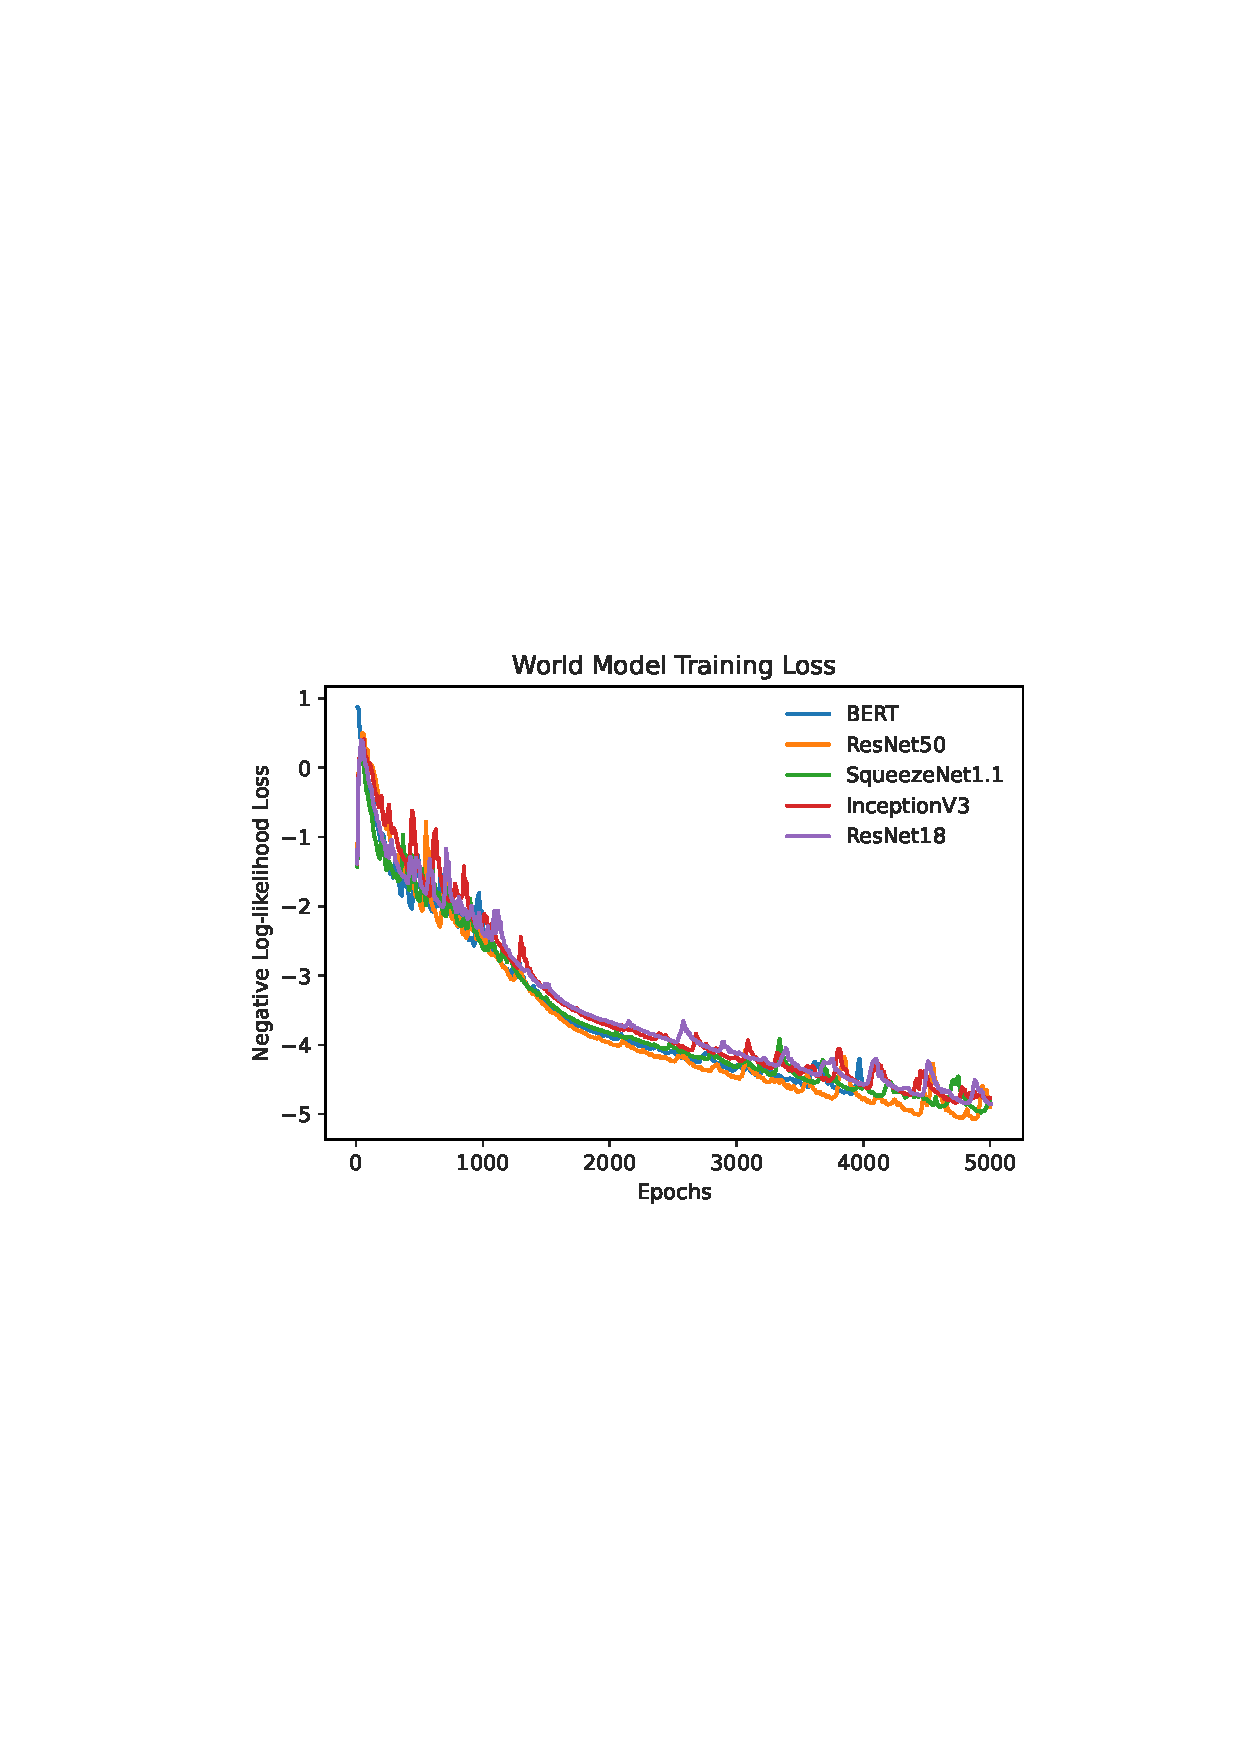
\includegraphics[width=1\columnwidth]{sections/5evaluation/images/mb_training_loss.png}
  \caption[Log-likelihood loss of world models]{Plot}
  \label{fig:eval:world-model-loss}
\end{figure}

We also show the convergence of the world model during training in figure \ref{fig:eval:world-model-loss} which is a plot of the log-likelihood loss per training epoch for each graph. We used the same hyperparameters for training each world model. Notably, we used decayed the learning rate of the course of 2000 epochs with the TensorFlow polynomial decay policy. The MDN-RNN is trained with 8 Gaussians and 256 hidden units, all other hyperparameters used in training the MDN-RNN world model are the same as those used by Ha and Schmidhuber \cite{ha2018worldmodels}, unless otherwise stated.

\begin{figure}[ht]
  \centering
  \includegraphics[width=1\columnwidth]{sections/5evaluation/images/mb_ctrl_training_reward.png}
  \caption[Predicted epoch reward during training of agent in world model]{Plot, temperature = 1}
  \label{fig:eval:world-model-pred-reward}
\end{figure}

Figure \ref{fig:eval:world-model-pred-reward} shows the reward (decrease in estimated runtime) for each graph as predicted by the world model during training. As the tested graphs have a wide range of epoch rewards, we perform min-max normalisation to scale the plots into the same range. We observe the same results as figure \ref{fig:eval:world-model-runtimes} in which the optimisations applied to BERT during training results in the optimal graph found after 700 epochs. On the other hand, graphs such as ResNet 18/50 are less stable during training with a high epoch to epoch variation in rewards.

[TODO temperature sweep]

\section{Discussion}

% Model-free agent rewards + performance
% Memory used by graphs after performing optimisation
% Temperature sweep for MB agents
% Hyperparameter search
% Reward prediction for model-based method
  % --> Separate reward pred network
  % --> Mask pred network?
% Heatmap plot of graph xfers
% Show sample graph xfers graphically

\chapter{Conclusion and Future Work}

\section{Conclusion}

In this work, we have shown the result of applying deep reinforcement learning techniques to the task of optimising deep neural networks. Our approach uses RL agents to select optimal actions that optimise the computation graphs with the goal of improving on-device runtime. We performed experiments that show RL agents decreased the runtime on all of the five test graphs, each of which had unique properties and architectures. Notably, we provide evidence to support our claim that it is possible to learn a world-model of the environment which is sufficiently accurate to enable the end-to-end training of an agent inside a fully imagined world-model. Furthermore, by leveraging the prior work by Jia et al., we developed a deeply instrumented environment in which we can train model-free agents and train world-models for model-based agents.

In addition, this work has highlighted that the performance of model-based agents trained inside a world-model is highly dependent on the accuracy of the model. Inaccuracies in the model, can lead to compounding errors and thus the agent choosing sub-optimal, or invalid, actions that diverges the imaged state from the true environment state. Therefore, there are still significant fundamental difficulties in training stable, accurate world-models that can simulate the true environment; if one can train such a model by carefully tuning hyperparameters, we can gain substantial benefits through increased sample efficiency and decreased training time.

\section{Future Work}

% In this work, we used a relatively simple mapping procedure to convert the TASO graph representation into a format that can be utilised by the \texttt{graph\textunderscore nets} package. 
% - Mapping computation graphs to GNN

In this work, we have presented an approach to using message-passing neural networks to exploit the relational biases in the graph structure of the input and produce a embedding of the graph in latent space. One possible direction for future work is to investigate the use of graph auto-encoders \cite{battaglia2018relational} to produce a reconstructed graph which can be used for planning. Recent work \cite{hafner2018learning, sekar2020planning} has shown that using an accurate world-model, we can exploit the model to plan our actions into the future state space to gain higher performance than would be possible using single-step state predictions.

Model-based reinforcement learning is an active area of research and recent work has shown significant improvement in the performance of model-based methods on tasks in which model-free methods traditionally excel. \citet{hafner2021mastering} show that using discrete world models that learn directly in latent space using planning, actor-critic agents can surpass model-free in the Atari environment. We propose that a future direction of work can be to investigate the use of discrete world models with actor-critic agents that offer greatly stability during training and learn more accurate world models which is especially critical to the performance of agents in system environments.

%\appendix
%\singlespacing

\bibliographystyle{plainnat} 
\bibliography{ref} 

\end{document}
